\pagebreak
\chapter{Results}
\section{Tree Creation}
A tree is generated from a certain area. To display and compare the differences a graph recreation algorithm was written. Therefore the printed result is also a nearly equal graph. Figure \ref{fig:tree_example} is a selected cluster before the tree creation. Figure \ref{fig:tree_example_after} is the recreated graph from the tree. The grid behind the recreated subgraph is rotated. This rotation depends on the angle of the start edge.

\begin{figure}[ht]
    \centering
    \begin{subfigure}[b]{0.55\textwidth}
        \begin{mdframed}[style=mdthight]
            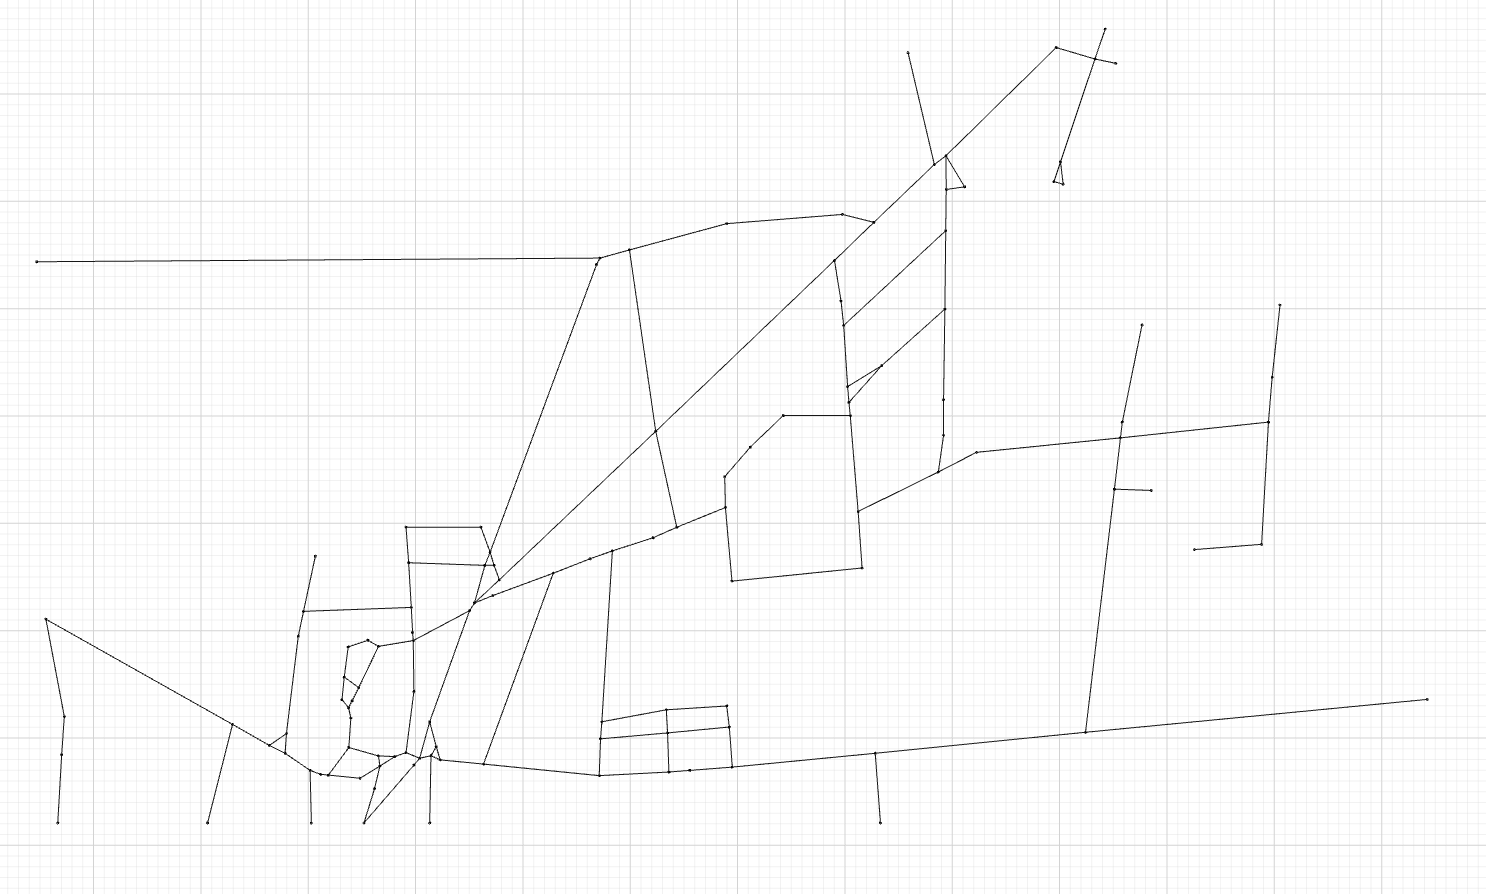
\includegraphics[width=\textwidth]{tree_before.png}
        \end{mdframed}
        \caption{Subgraph of Weimar}
        \label{fig:tree_example}
    \end{subfigure}
    \quad
    \begin{subfigure}[b]{0.55\textwidth}
        \begin{mdframed}[style=mdthight]
            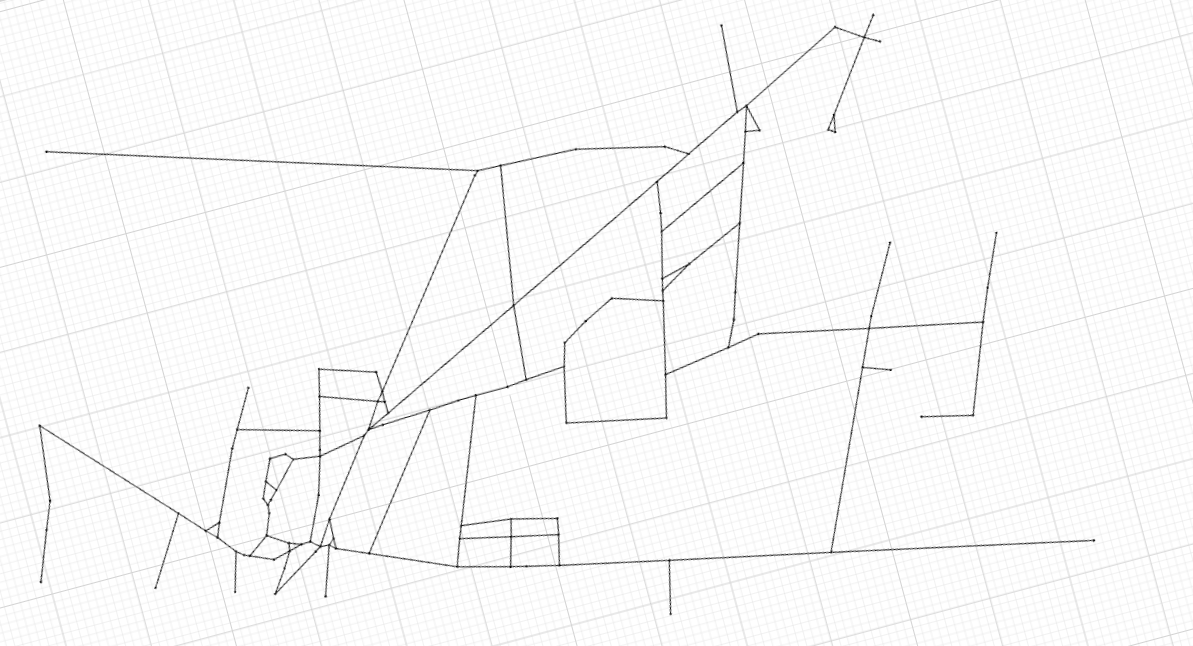
\includegraphics[width=\textwidth]{tree_after.png}
        \end{mdframed}
        \caption{Recreated Subgraph from tree of Weimar}
        \label{fig:tree_example_after}
    \end{subfigure}
    \caption{Subgraph before \ref{fig:tree_example} and after \ref{fig:tree_example_after} tree creation}
\end{figure}

\FloatBarrier
\section{K-Means}
The K-Means algorithm assigns points by using random centroids and assign all nearest points to them. Then the centroids are moved into the centre of their assigned points. This process is repeated till no point is moved.

The implementation in CPlan \ref{CPlan} produced the following image \ref{fig:KmeansGenerated} based on the city of Weimar. All streets in one cluster are marked with the same colour, the transitions between clusters are marked black.

\subsection{Connected Cluster Problem}
As presumed the resulting subgraph had unexpected transitions between clusters. This means some clusters were not connected. In the image \ref{fig:KmeansProblem} the result can be observed in the read circle where only one point is marked as outer cluster. The two black lines represent the cluster transitions.

\begin{figure}[!ht]
    \centering
    \begin{mdframed}[style=mdthight, userdefinedwidth=0.55\textwidth, align=center]
        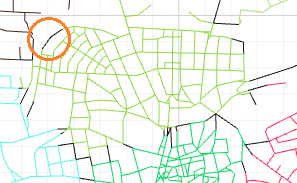
\includegraphics[width=\textwidth]{clusteranalysis_kmeans_problem.png}
    \end{mdframed}
    \caption{Problem of K-Means clustering
        \label{fig:KmeansProblem}}
\end{figure}

\subsection{Connected Cluster Results} \label{sec:K-Means_shortest_path}
To problem was then solved by using a \gls{APSP} algorithm like Dijkstra or Floyd-Warshall. In the following figure \ref{fig:Kmeansshortestp} every cluster is a connected subgraph.

\begin{figure}
    \centering
    \begin{mdframed}[style=mdthight]
        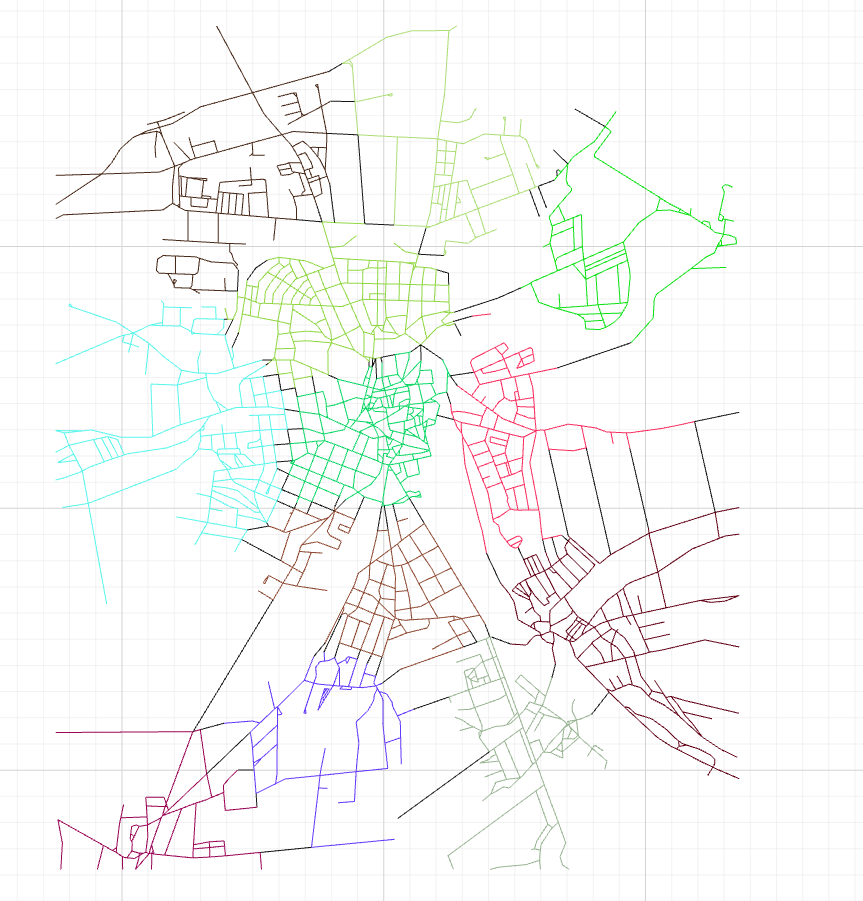
\includegraphics[width=\textwidth]{clusteranalysis_kmeans_result.png}
    \end{mdframed}
    \caption{K-Means cluster analysis of Weimar \label{fig:KmeansGenerated}}
\end{figure}

\begin{figure}
    \centering
    \begin{mdframed}[style=mdthight]
        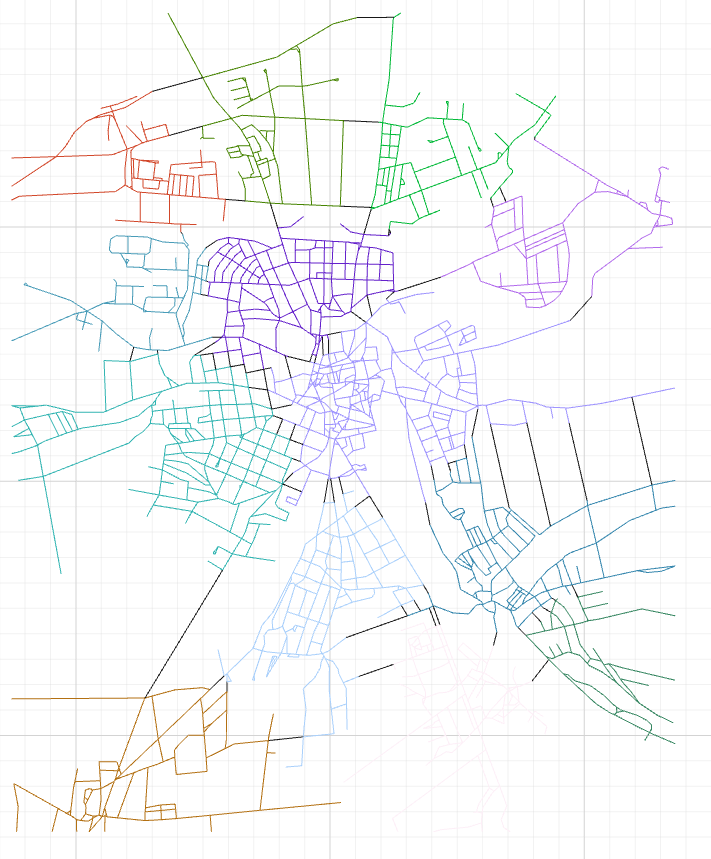
\includegraphics[width=\textwidth]{clusteranalysis_kmeansExt_result.png}
    \end{mdframed}
    \caption{K-Means clustering with shortest path\label{fig:Kmeansshortestp}}
\end{figure}

\section{Single-Linkage Result}
The figure \ref{fig:SingleLinkage} shows the result of a hierarchical cluster analysis of Weimar using the single linkage reduction formula. The used distance function $d(i, j)$ was the shortest distance from $i$ to $j$ in the street graph. As it is clearly visible when looking at the result, this way of cluster analysis is not creating the desired output. There is one huge cluster in the middle and many one-node clusters at the border of the city.

The problem is caused by the used reduction formula. Single linkage uses the minimal distance between all nodes of the compared clusters. This leads to the creation of clusters, where all roads which connect two clusters are long. In a city, where there are multiple (direct and indirect) connections from one junction to another most of the time, this tends to create one-node clusters for nodes, which are connected to the city by a single long road.

\begin{figure}
    \centering
    \begin{mdframed}[style=mdthight]
        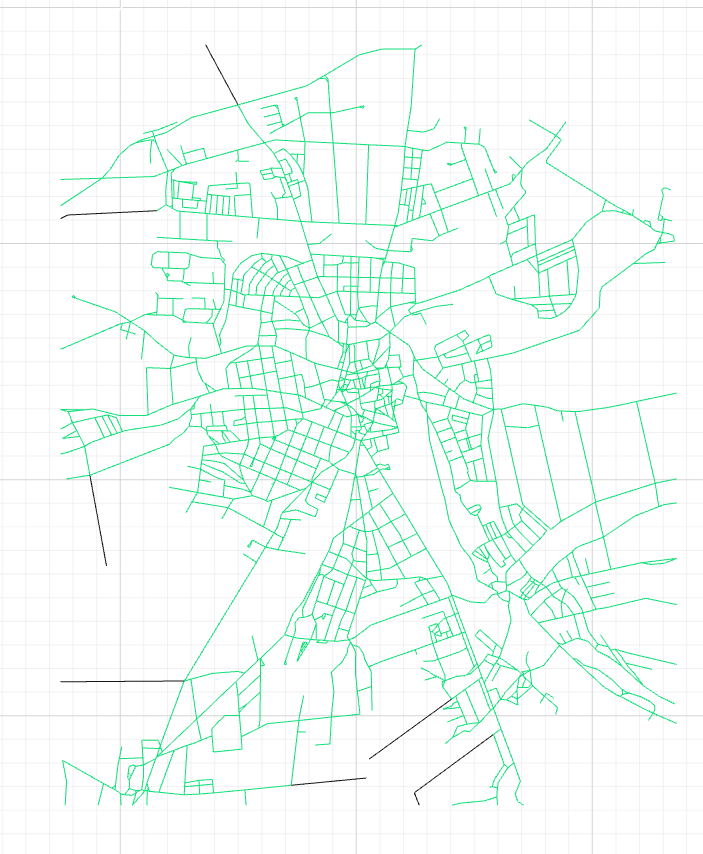
\includegraphics[width=\textwidth]{clusteranalysis_singlelinkage.png}
    \end{mdframed}
    \caption{Single-Linkage hierarchical cluster analysis of Weimar\label{fig:SingleLinkage}}
\end{figure}

\section{UPGMA and WPGMA Result}
\label{sec:UPGMAandWPGMA}
The figures \ref{fig:hierarchical_clustering_upgma} and \ref{fig:hierarchical_clustering_wpgma} show the result of hierarchical cluster analysis using the \acrshort{UPGMA}, or respectively the \acrshort{WPGMA} reduction formula. The same distance function $d(i, j)$ as in the single linkage solution was used (shortest distance from $i$ to $j$ in the street graph).

%TODO: Compare, conclusions?

\begin{figure}
    \centering
    \begin{mdframed}[style=mdthight]
        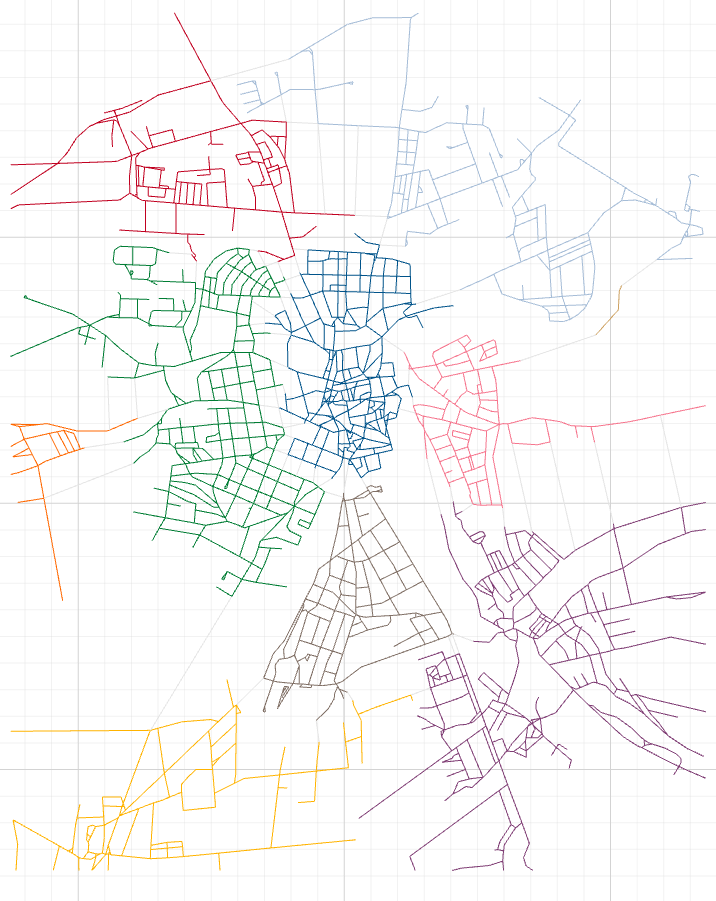
\includegraphics[width=\textwidth]{hierarchical_clustering_upgma.png}
    \end{mdframed}
    \caption{UPGMA hierarchical cluster analysis of Weimar\label{fig:hierarchical_clustering_upgma}}
\end{figure}


\begin{figure}
    \centering
    \begin{mdframed}[style=mdthight]
        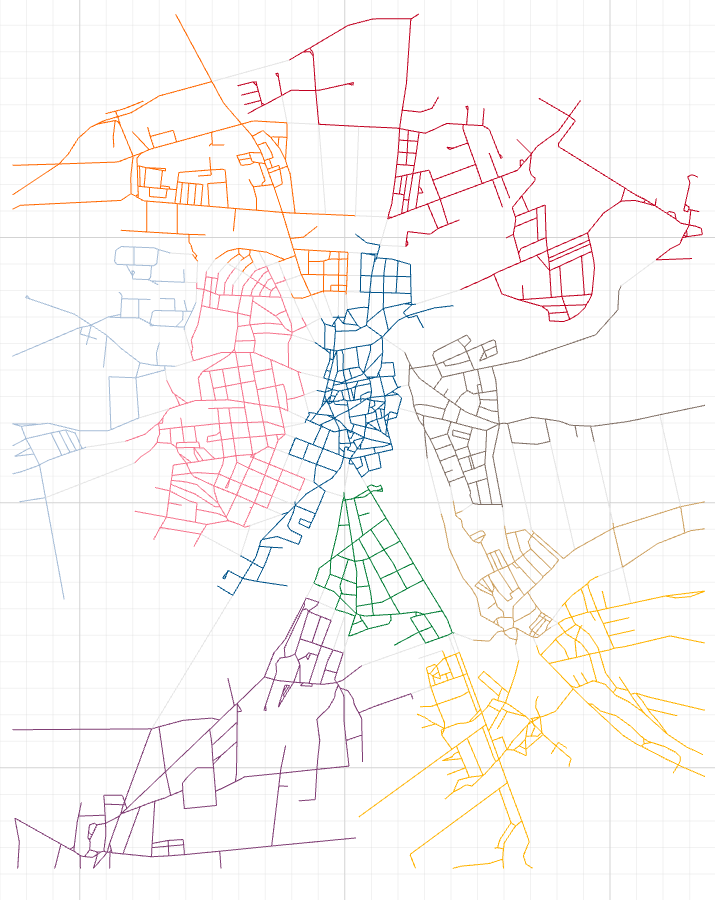
\includegraphics[width=\textwidth]{hierarchical_clustering_wpgma.png}
    \end{mdframed}
    \caption{WPGMA hierarchical cluster analysis of Weimar\label{fig:hierarchical_clustering_wpgma}}
\end{figure}
